%%%%%%%%%%%%%%%%%%%%%%%%%%%%%%%%%%%%%%%%%%%%%%%%%%%%%%%%%%%%%%%%%%%%%%%%
% Plantilla TFG/TFM
% Escuela Politécnica Superior de la Universidad de Alicante
% Realizado por: Jose Manuel Requena Plens
% Contacto: info@jmrplens.com / Telegram:@jmrplens
%%%%%%%%%%%%%%%%%%%%%%%%%%%%%%%%%%%%%%%%%%%%%%%%%%%%%%%%%%%%%%%%%%%%%%%%

\chapter{Metodología}
\label{metodologia}
La metodología de este proyecto se basa en algunas metodologías ágiles estudiadas en las asignaturas de la carrera dedicadas a ello, es una metodología iterativa. Esto nos permite a mi tutor y a mí, ver en qué partes necesito más ayuda y en cuáles podemos avanzar más rápido, pudiendo así adaptar perfectamente la velocidad del desarrollo en cada iteración.
\begin{figure}[h]
	\centering
	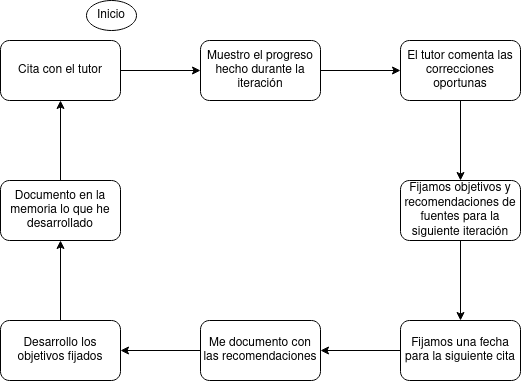
\includegraphics[width=15cm]{archivos/imagenes/diagrama-de-metodologia.png}
	\caption{Metodología de trabajo seguida durante el desarrollo.}
	\label{diagrama de metodologia}
\end{figure}

El ciclo comienza en el cuadrado superior izquierdo, y salvo la primera iteración, en la que no hubo que mostrar el progreso, y por lo tanto no hubo nada que corregir, y en la última iteración, que no hubo que concertar una futura cita, el resto de iteraciones siguieron el patrón que se puede ver en la figura \ref{diagrama de metodologia}.

Todas las iteraciones duran entre 3 y 4 semanas. Para cada iteración se concierta una cita entre el tutor y el alumno, se pone un objetivo de trabajo y una fecha para la próxima quedada. En esta reunión se exponen los trabajos concretados en la anterior, que han de estar finalizados y se propondrán los siguientes.
\\
Cada iteración o sprint consta de una parte de formación, en la que el alumno, orientado por el tutor, adquiere conocimientos sobre lo que se va a trabajar\footnote{Esto puede tratarse tanto de vídeos formativos como de libros u otras lecturas recomendadas.}, y lo pone en práctica en el proyecto. Finalmente, todo lo hecho durante ese sprint se documenta en el documento del \gls{tfg} y se muestra el progreso al tutor, quién valora el trabajo y propone alguna corrección en caso de ser necesaria.

\section{Control de versiones}
Para gestionar el control de versiones usaré la famosa herramienta Git\footnote{Software creado por Linus Torvalds para el control de versiones.} debido a lo extendido que está, tanto en el mundo laboral, como para uso personal, y lo fácil que es de usar a través de plataformas como GitHub\footnote{Plataforma de Microsoft, utilizada comúnmente para compartir código de forma abierta en Internet, que implementa el control de versiones de Git.}. Esto me permite compartir el código fácilmente con mi tutor, tener un respaldo en la nube de mi trabajo, y además volver a una versión anterior del código estable, en el caso de que cambie cosas que no debería haber hecho.
\\
El momento en el que tomo una instantánea del código, o como se le conoce hacer ``commit'', es al acabar una idea previamente planteada. Por ejemplo, si quiero implementar el funcionamiento de la gravedad: pienso cómo se haría, lo implemento y compruebo que funciona, y el proyecto ya está listo para hacer ``commit''. Si posteriormente se encuentra algún defecto se modificará el código y se hará otro ``commit'' con un mensaje descriptivo, comentando cuál era el defecto arreglado, y esto ayudará a evitar errores como borrar o modificar partes del código que no debía. 

\section{Herramientas de trabajo}
\label{herramientas}
A parte de las anteriormente mencionadas \textbf{Git} y \textbf{GitHub}, voy a utilizar las siguientes herramientas:
\begin{itemize}
    \item \textbf{Visual Studio Code:} Se trata de un editor de texto creado por Microsoft, derivado de su \gls{ide}\footnote{Entorno de desarrollo integrado en español, herramienta que te ayuda en tareas de programación como auto-completar código, compilar, etc.} Visual Studio, pero open source, multiplataforma y simplificado. Dispone de un montón de extensiones que lo hacen compatible con cualquier lenguaje que disponga de una.
    \item \textbf{TeXstudio:} Este \gls{tfg} está siendo escrito en \LaTeX por lo que es necesario un editor para facilitar el uso del lenguaje, con correcciones y para poder pre-visualizar el documento final.
    \item \textbf{xelatex:} Es el compilador que utiliza TeXstudio para compilar los documentos \LaTeX.
    \item \textbf{Gimp:} Herramienta de creación y edición de imágenes, útil para poder crear o modificar las imágenes necesarias para ilustrar algunas partes del \gls{tfg}.
    \item \textbf{draw.io:} Aplicación online para la creación de diagramas, que también usaré para ilustrar el \gls{tfg}.
    \item \textbf{g++:} Compilador de C++ desarrollado por GNU para compilar en sistemas basados en Unix.
    \item \textbf{clang++:} Otro compilador de C++ alternativo, ya que, aunque siguen el estándar de C++, uno te puede dar los errores que otro no, o mostrarlos de una forma distinta, y eso puede ayudar entenderlos o evitar errores en el futuro.
    \item \textbf{gdb:} Un depurador de C++, útil para encontrar errores en el código. Es compatible con Visual Studio Code, por eso, y su gran facilidad de uso es el elegido. 
    \item \textbf{make:} Herramienta de gestión de dependencias, para compilar y recompilar de forma automática el código y generar el ejecutable.
    \item \textbf{Arch Linux:} Sistema operativo, basado en Linux, que utilizo en mi portátil para el desarrollo del \gls{tfg}.
\end{itemize}